\documentclass[a4paper,10pt]{article}

\usepackage[utf8]{inputenc}
\usepackage{fontenc}
\usepackage{graphicx}
\usepackage{hyperref}
\usepackage{multirow}
\usepackage{titling}
\usepackage{amssymb}
\usepackage{amsmath}
\usepackage{geometry}
\geometry{verbose,a4paper, tmargin=25mm, bmargin=25mm, lmargin=25mm, rmargin=25mm}

\title{Binary Timeseries File Format Specification}
\author{Jonathan Schilling}
\date{\today}

\usepackage{attachfile2}
\attachfilesetup{color=1 0 0,
                 author={\theauthor},
                 subject={Attached File}}

\begin{document}
\maketitle

\section{Scope}\label{sec:scope}

This is the specification for a really simple binary file format for storing a regularly-spaced sequence of single-channel measurement data
in an efficiently writeable and readable format.
The basic assumption is that the time axis~$t_i$ of a series of $N$~measurements can be computed on the fly from the array indices:
\begin{equation}
  t_i = t_0 + i \cdot \Delta t \quad \mathrm{for} \quad i = 0, 1, ..., (N-1) \quad ,
\end{equation}
where $t_0$ is the (reference) timestamp of the first sample and $\Delta t$ is the sampling interval.

The data values $y_i$ are stored as raw values $\hat{y}_i$, optionally with an offset~$o$ and a scaling factor~$s$:
\begin{gather}
\begin{aligned}
  y_i & = &             \hat{y}_i & \quad \mathrm{for} \quad i = 0, 1, ..., (N-1) & \mathrm{without~scaling,} \\
  y_i & = & o + s \cdot \hat{y}_i & \quad \mathrm{for} \quad i = 0, 1, ..., (N-1) & \mathrm{with~scaling.}
\end{aligned}
\end{gather}
The number of samples is limited by the maximum value of the (signed 32-bit) \texttt{int} type, which is
\begin{equation}
  2^{31} - 1 = 2\,147\,483\,647 \approx 2.1 \cdot 10^9 \quad .
\end{equation}
In case of raw \texttt{double} values, the corresponding maximum file size is $(64 + 8 \cdot 2\,147\,483\,647)\,\mathrm{bytes} \approx 16\,\mathrm{GB}$,
where 64~bytes are reserved for the file header information.

Suppose an ADC samples at a given frequency $f$. Then, the sampling interval $\Delta t = f^{-1}$.
Using this time series file format, a maximum of $2^{31}-1$ samples can be stored, which then corresponds to a
total duration $T_\mathrm{max}$ of
\begin{equation}
  T_\mathrm{max} = (2^{31}-1) \cdot \Delta t \quad .
\end{equation}
For a $f = 1\,\mathrm{Mhz}$ sampling rate, $\Delta t = 1\,\mu\mathrm{s}$ and $T_\mathrm{max} \approx 2147\,\mathrm{s}$.

The recommended file name extension for Binary Timeseries files is \texttt{*.bts}.

\section{Definitions}\label{sec:definitions}
In Tab.~\ref{tab:data types} you find an overview of the types for raw data considered in this specification.
\begin{table}[htbp]
 \centering
 \begin{tabular}{|c|c|c|c|c|c|}
    \hline
    type            & size in bytes & identifier value & ok for time & ok for scaling & ok for data \\
    \hline
    \textit{None}   & 0             & 0                & no          & yes            & no          \\
    \hline                                                                            
    \texttt{byte}   & 1             & 1                & no          & yes            & yes         \\
    \hline                                                                            
    \texttt{short}  & 2             & 2                & no          & yes            & yes         \\
    \hline                                                                            
    \texttt{int}    & 4             & 3                & no          & yes            & yes         \\
    \hline                                                                            
    \texttt{long}   & 8             & 4                & yes         & yes            & yes         \\
    \hline                                                                            
    \texttt{float}  & 4             & 5                & no          & yes            & yes         \\
    \hline                                                                            
    \texttt{double} & 8             & 6                & yes         & yes            & yes         \\
    \hline
 \end{tabular}
 \caption{Data types considered relevant for time series data.}
 \label{tab:data types}
\end{table}

The first column lists the Java-style name of the given types.
In the second column, the size of the corresponding type in bytes is listed.
The third column lists the numeric value of the \texttt{dtype} bytes identifying the type of data in the file (see below).
The last three columns tell you if a given type can be used to specify the time axis (ok for time),
the scaling of the raw data (ok for scaling) and the raw data values (ok for data).

Throughout this document, the data types refer to the signed version of these. Unsigned versions of the data types are not
considered here, as they are not available in certain programming languages (e.g. Java).

\section{File Structure}\label{sec:file_structure}
The contents of the files are structured as shown in Tab.~\ref{tab:structure}.
\begin{table}[htbp]
 \centering
 \begin{tabular}{|c|c|c|c|c|}
    \hline
    offset & size             & type                             & allowed values    & description \\
    \hline                                                                                 
    0      & 2                & \texttt{short}                   & 1                 & used to verify correct endianess  \\
    \hline                                                                                 
    2      & 1                & \texttt{byte}                    & 4 or 6            & data type of time: 4 (long) or 6 (double) \\
    \hline                                                                                 
    3      & 8                & \texttt{long} or \texttt{double} & \textit{any}      & $t_0$: reference timestamp \\
    \hline                                                                                 
    11     & 8                & \texttt{long} or \texttt{double} & \textit{any}      & $\Delta t$: time interval between two samples \\
    \hline                           
    19     & 1                & \texttt{byte}                    & 0 ... 6           & data type of scaling for data values; \\
     ~     & ~                &      ~                           &                   & 0 (\textit{None}) indicates that scaling is disabled  \\
    \hline                           
    [20]   & 8                & \textit{varying}                 & \textit{any}      & offset $o$ of data values \\
    \hline                                                                                 
    [28]   & 8                & \textit{varying}                 & \textit{any}      & scaling factor $s$ for data values \\
    \hline                                                                                 
    36     & 23               & \textit{reserved}                & \textit{reserved} & reserved for future use, e.g. units \\
    \hline                                                                                 
    59     & 1                & \texttt{byte}                    & 1 ... 6           & dtype of raw data: 1 (byte) to 6 (double) \\
    \hline                                                              
    60     & 4                & \texttt{int}                     & $> 0$             & number $N$ of data values \\
    \hline
    64     & \textit{varying} & \textit{varying}                 & \textit{any}      & data values $\hat{y}_i$ of type given by dtype \\
    \hline
 \end{tabular}
 \caption{Structure of the binary timeseries files.
 The values in the columns ``offset'' and ``size'' are in bytes.
 The rows where the offset is in [ ] are not valid and should contains zeros in the file if no scaling for the data values is used.}
 \label{tab:structure}
\end{table}

The first field at offset 0 in the file is a \texttt{short}, which is always 1.
It should be read using a \texttt{readShort()} or similar function, which implicitly assumes the system's endianess.
Then it should be checked if the returned value is $1$ or $256$.
In the latter case, the endianess of the reading method is wrong and needs to be flipped in order to proceed.

The next field at offset 2 defines the data type of the time axis definition values $t_0$ and $\Delta t$.
If it is equal to 3, the time definition is given as \texttt{long}.
If it is equal to 5, the time definition is given as \texttt{double}.
No assumption should be made on the unit of these values, although it is recommended to reserve \texttt{double} for seconds and
\texttt{long} for nanoseconds.

The next field at offset 3 defines the reference timestamp $t_0$ and has to be read as a \texttt{long} or \texttt{double},
depending on the value read at offset 2.
The next field at offset 11 defines the sampling interval $\Delta t$ and has to be read as a \texttt{long} or \texttt{double},
depending on the value read at offset 2.
The time axis definition values $t_0$ and $\Delta t$ always have to be of the same data type and should use the same unit.

The field at offset 19 defines the data type of the scaling parameters $o$ and $s$ to come.
If its value is zero, no scaling is used and the next sixteen bytes can be ignored.

At offset 20, the constant offset $o$ of the raw data is stored. Its size can range from one byte to at most eight bytes
and it is always stored from offset 20 on; the remaining (unused) bytes in case of a type smaller than 8 bytes are ignored and should be written as zeros.
Right after the data offset value, at an offset of 28, the scaling factor $s$ is stored.
Its size can range from one byte to at most eight bytes
and it is always stored from offset 28 on; the remaining (unused) bytes in case of a type smaller than 8 bytes are ignored and should be written as zeros.
The scaling parameters $o$ and $s$ always have to be of the same data type and should use the same unit.

The bytes at offsets 36 to 58 are reserved for future use.

The next field at offset 59 defines the data type of the raw data.
Right after the raw data type, at an offset of 60, the number of data values $N$ to come is stored.
From offset 64 on, the raw data values $\hat{y}_i$ are stored, which have to be read as the data type defined by the value at offset 59.

\section{Subset Reading}\label{sec:subset_reading}
The main goal of this file format is to allow easy and fast reading of subsets of the whole time series data.
Having an equally spaced time axis allows to compute the data indices inside a given time interval and using the definitions in Sec.~\ref{sec:file_structure},
the offsets in the file can be computed for seeking to the computed position in the file and reading only from there on.

Suppose you have read $t_0$ and $\Delta t$ from the binary timeseries file header and now want to read all available samples
inside the interval $[t_l, t_u]$ where $t_l < t_u$ and the subscript $l$ ($u$) stand for \textit{lower} (\textit{upper}).
This situation is illustrated in Fig.~\ref{fig:timeAxis}
(\textattachfile[description={SVG version of Fig.~\ref{fig:timeAxis}}]{timeAxis.svg}{SVG},~\textattachfile[
                 description={EPS version of Fig.~\ref{fig:timeAxis}}]{timeAxis.eps}{EPS}).
\begin{figure}[htbp]
  \centering
  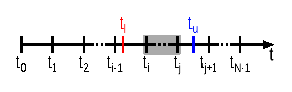
\includegraphics[width=0.6\textwidth]{timeAxis.eps}
  \caption{Time axis of a time series, where all data between $t_l$ and $t_u$ should be read.
  The resulting interval to be read includes indices from $i$ to $j$ and is indicated by the grey rectangle.}
  \label{fig:timeAxis}
\end{figure}

It is evident that the timestamps $t_l$ and $t_u$ are not necessarily aligned with the time axis of the available data.
Therefore, rounding has to be used to compute the indices of data:
\begin{itemize}
  \item \texttt{double} timestamps: $t_0, \Delta t \in \mathbb{R}_\mathrm{64\,bit}$
  \begin{gather}
   \begin{align}
    i & = \left\lceil  \frac{t_l - t_0}{\Delta t} \right\rceil  \in \mathbb{N} \\
    j & = \left\lfloor \frac{t_u - t_0}{\Delta t} \right\rfloor \in \mathbb{N}
   \end{align}
  \end{gather}
  \item \texttt{long} timestamps: $t_0, \Delta t \in \mathbb{Z}_\mathrm{64\,bit}$
  \begin{gather}
   \begin{align}
    i & = \frac{t_l - t_0 + \Delta t - 1}{\Delta t} \in \mathbb{N} \\
    j & = \qquad \frac{t_u - t_0}{\Delta t} \qquad  \in \mathbb{N}
   \end{align}
  \end{gather}
\end{itemize}
In case of the \texttt{long} timestamps, implicit computation of the floor of the division result is assumed.
Using these formulas, the relevant part of the file to be read starts at index $i$ and ends at index $j$.
Note that these formulas are only valid if $t_0 < t_l < t_u < t_{N-1}$ holds.








\section{Finalizing Remarks}
Implementations of this file format in Java and Python are available on GitHub:
\begin{center}
\href{https://github.com/jonathanschilling/BinaryTimeseries}{https://github.com/jonathanschilling/BinaryTimeseries}
\end{center}
The Java version is also available on Maven~Central:
\begin{verbatim}
<dependency>
  <groupId>de.labathome</groupId>
  <artifactId>BinaryTimeseries</artifactId>
  <version>1.0.1</version>
</dependency>
\end{verbatim}
The Python version is planned to be released on \texttt{PyPI}.\\
In case of questions or bug reports, please create an issue on GitHub:
\begin{center}
\href{https://github.com/jonathanschilling/BinaryTimeseries/issues}{https://github.com/jonathanschilling/BinaryTimeseries/issues}
\end{center}

\end{document}
